\begin{figure}[H]
\centering
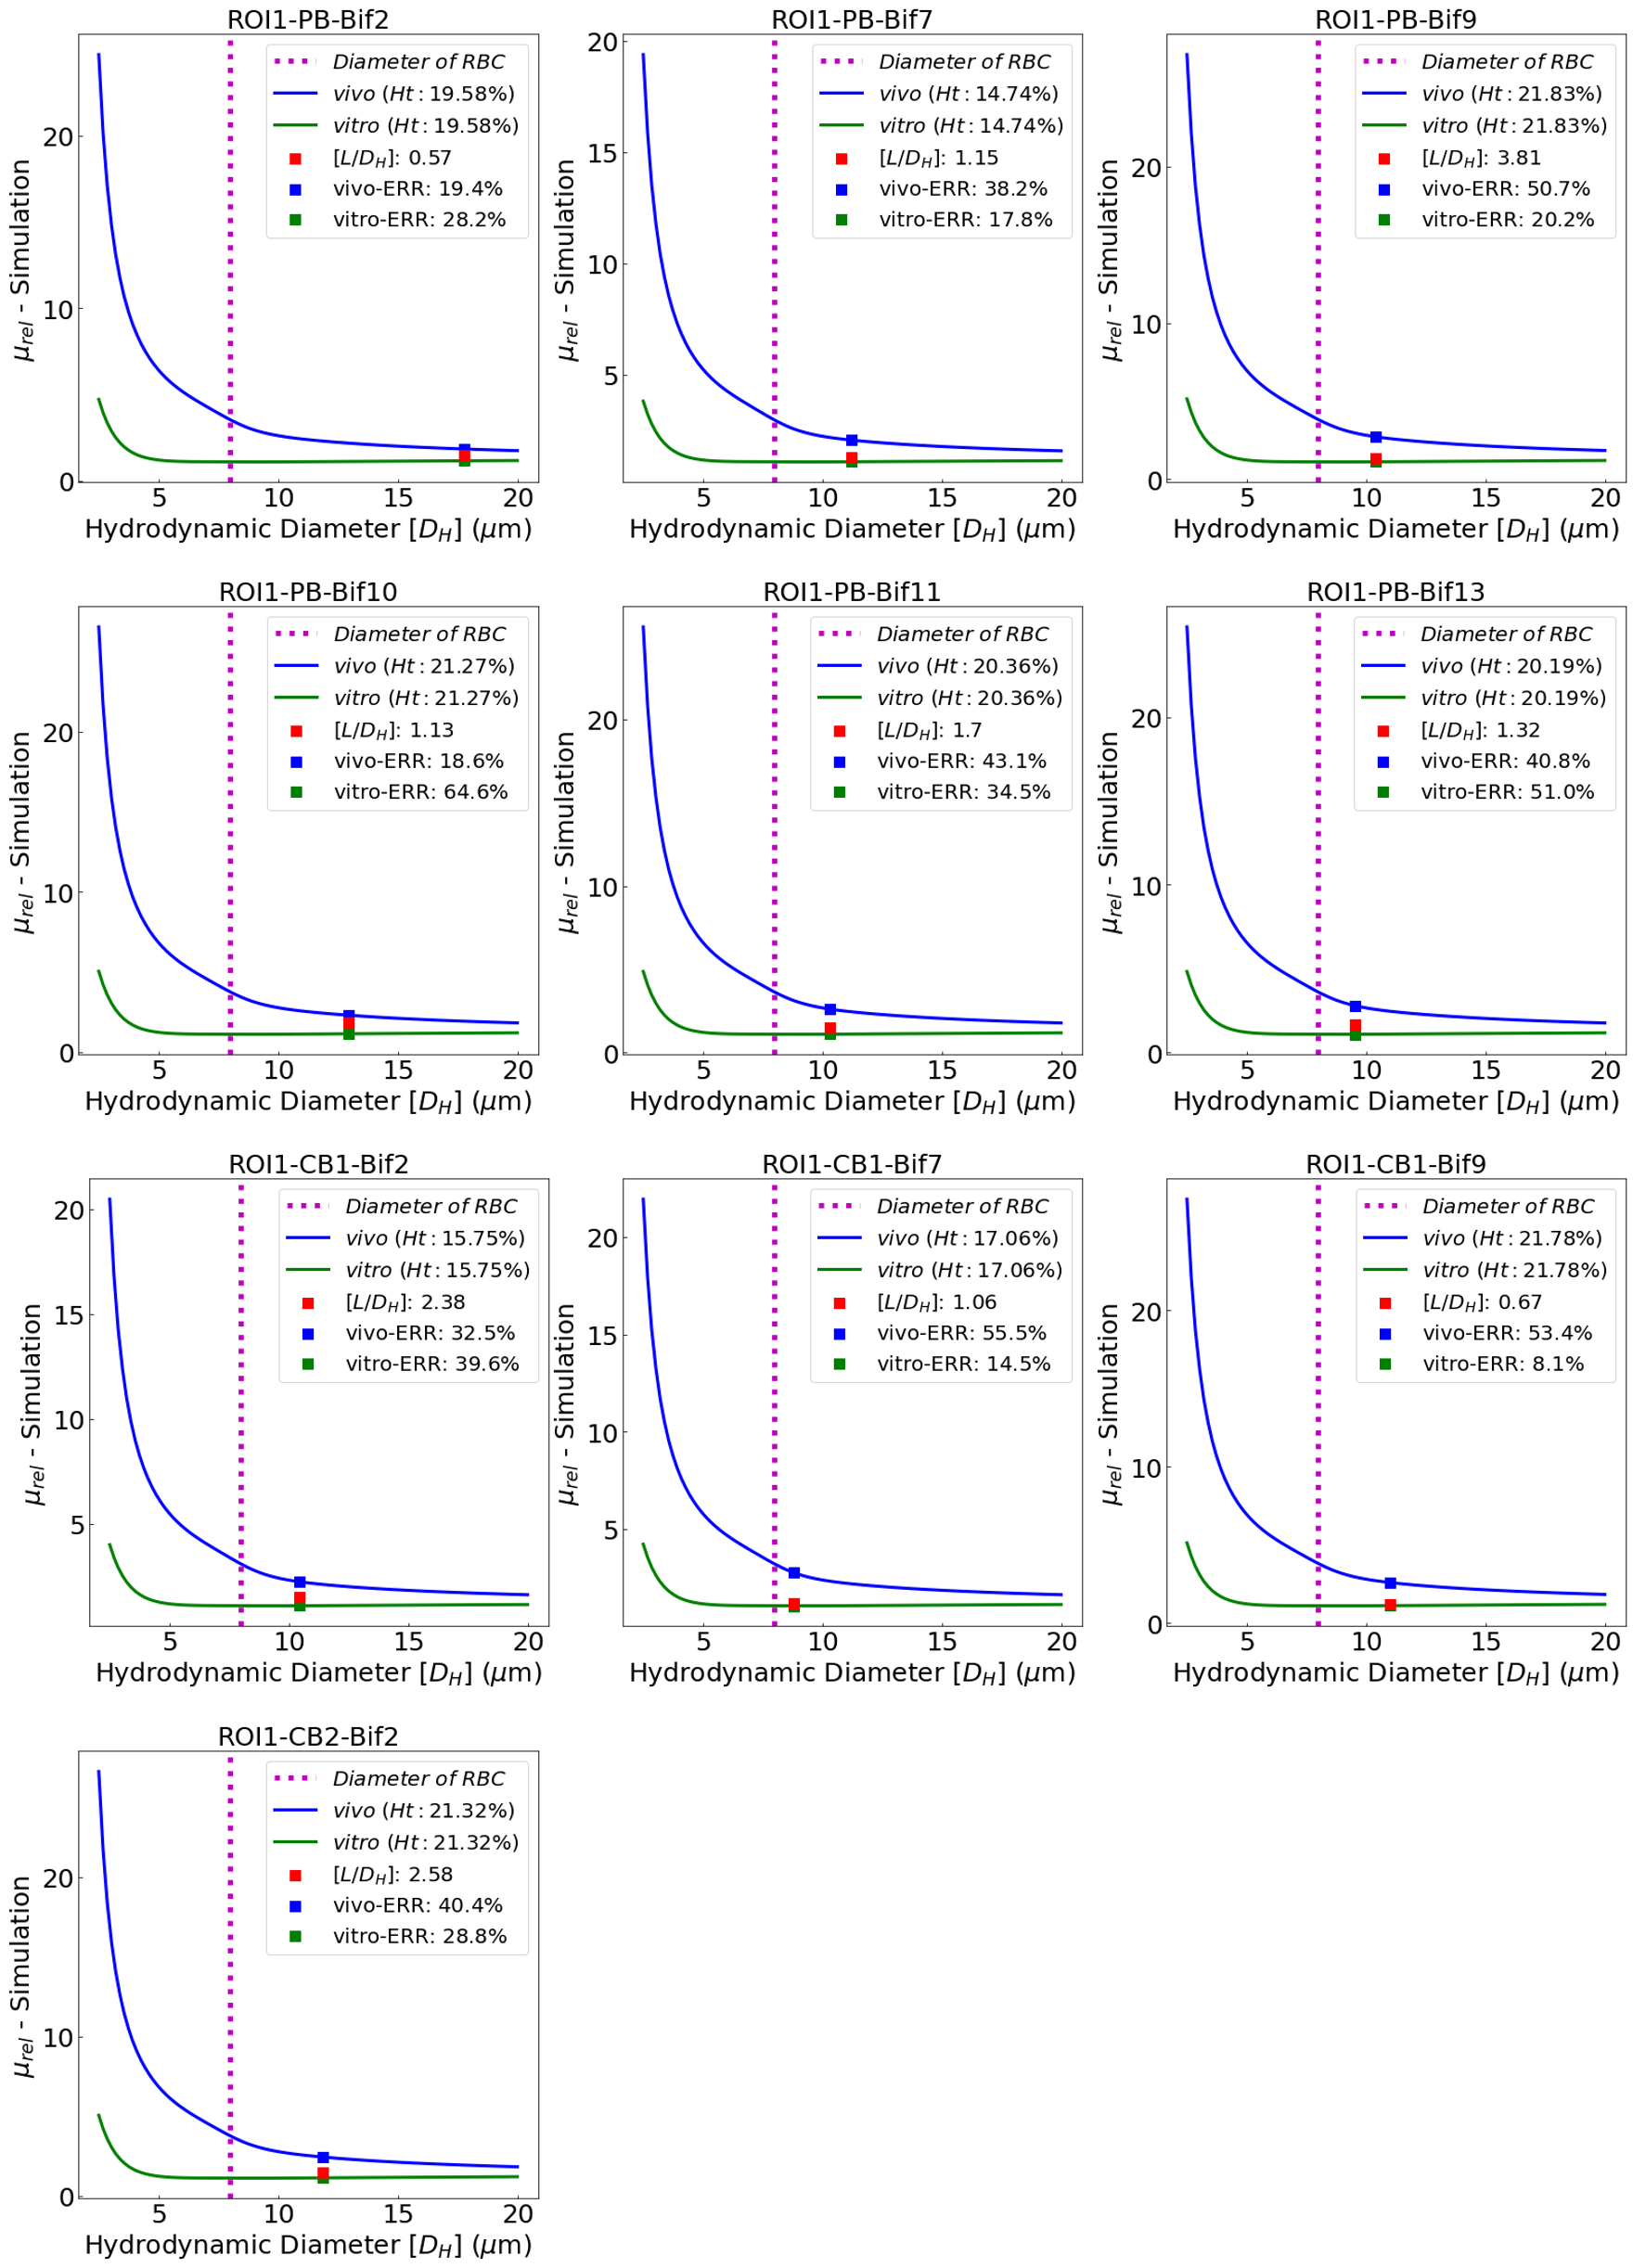
\includegraphics[width=0.925\textwidth]{images/DeviationsViscosity-ROI1.png}
\caption{\textit{Evaluation of non-zero haematocrit simulation data (red) against the empirical predictions (blue and green) from both in vivo and in vitro Pries Viscosity Models (solid lines) expressed as relative apparent viscosity ($\mu_{rel}$) against diameter (D$_{H}$) for each individual branch in ROI-1.(see Figure \ref{ROIs}a) The purple dotted line indicates the average diameter of a human RBC.} \label{DeviationsViscosity-ROI1}}
\end{figure}


\uselandscape
\begin{figure}[H]
\centering
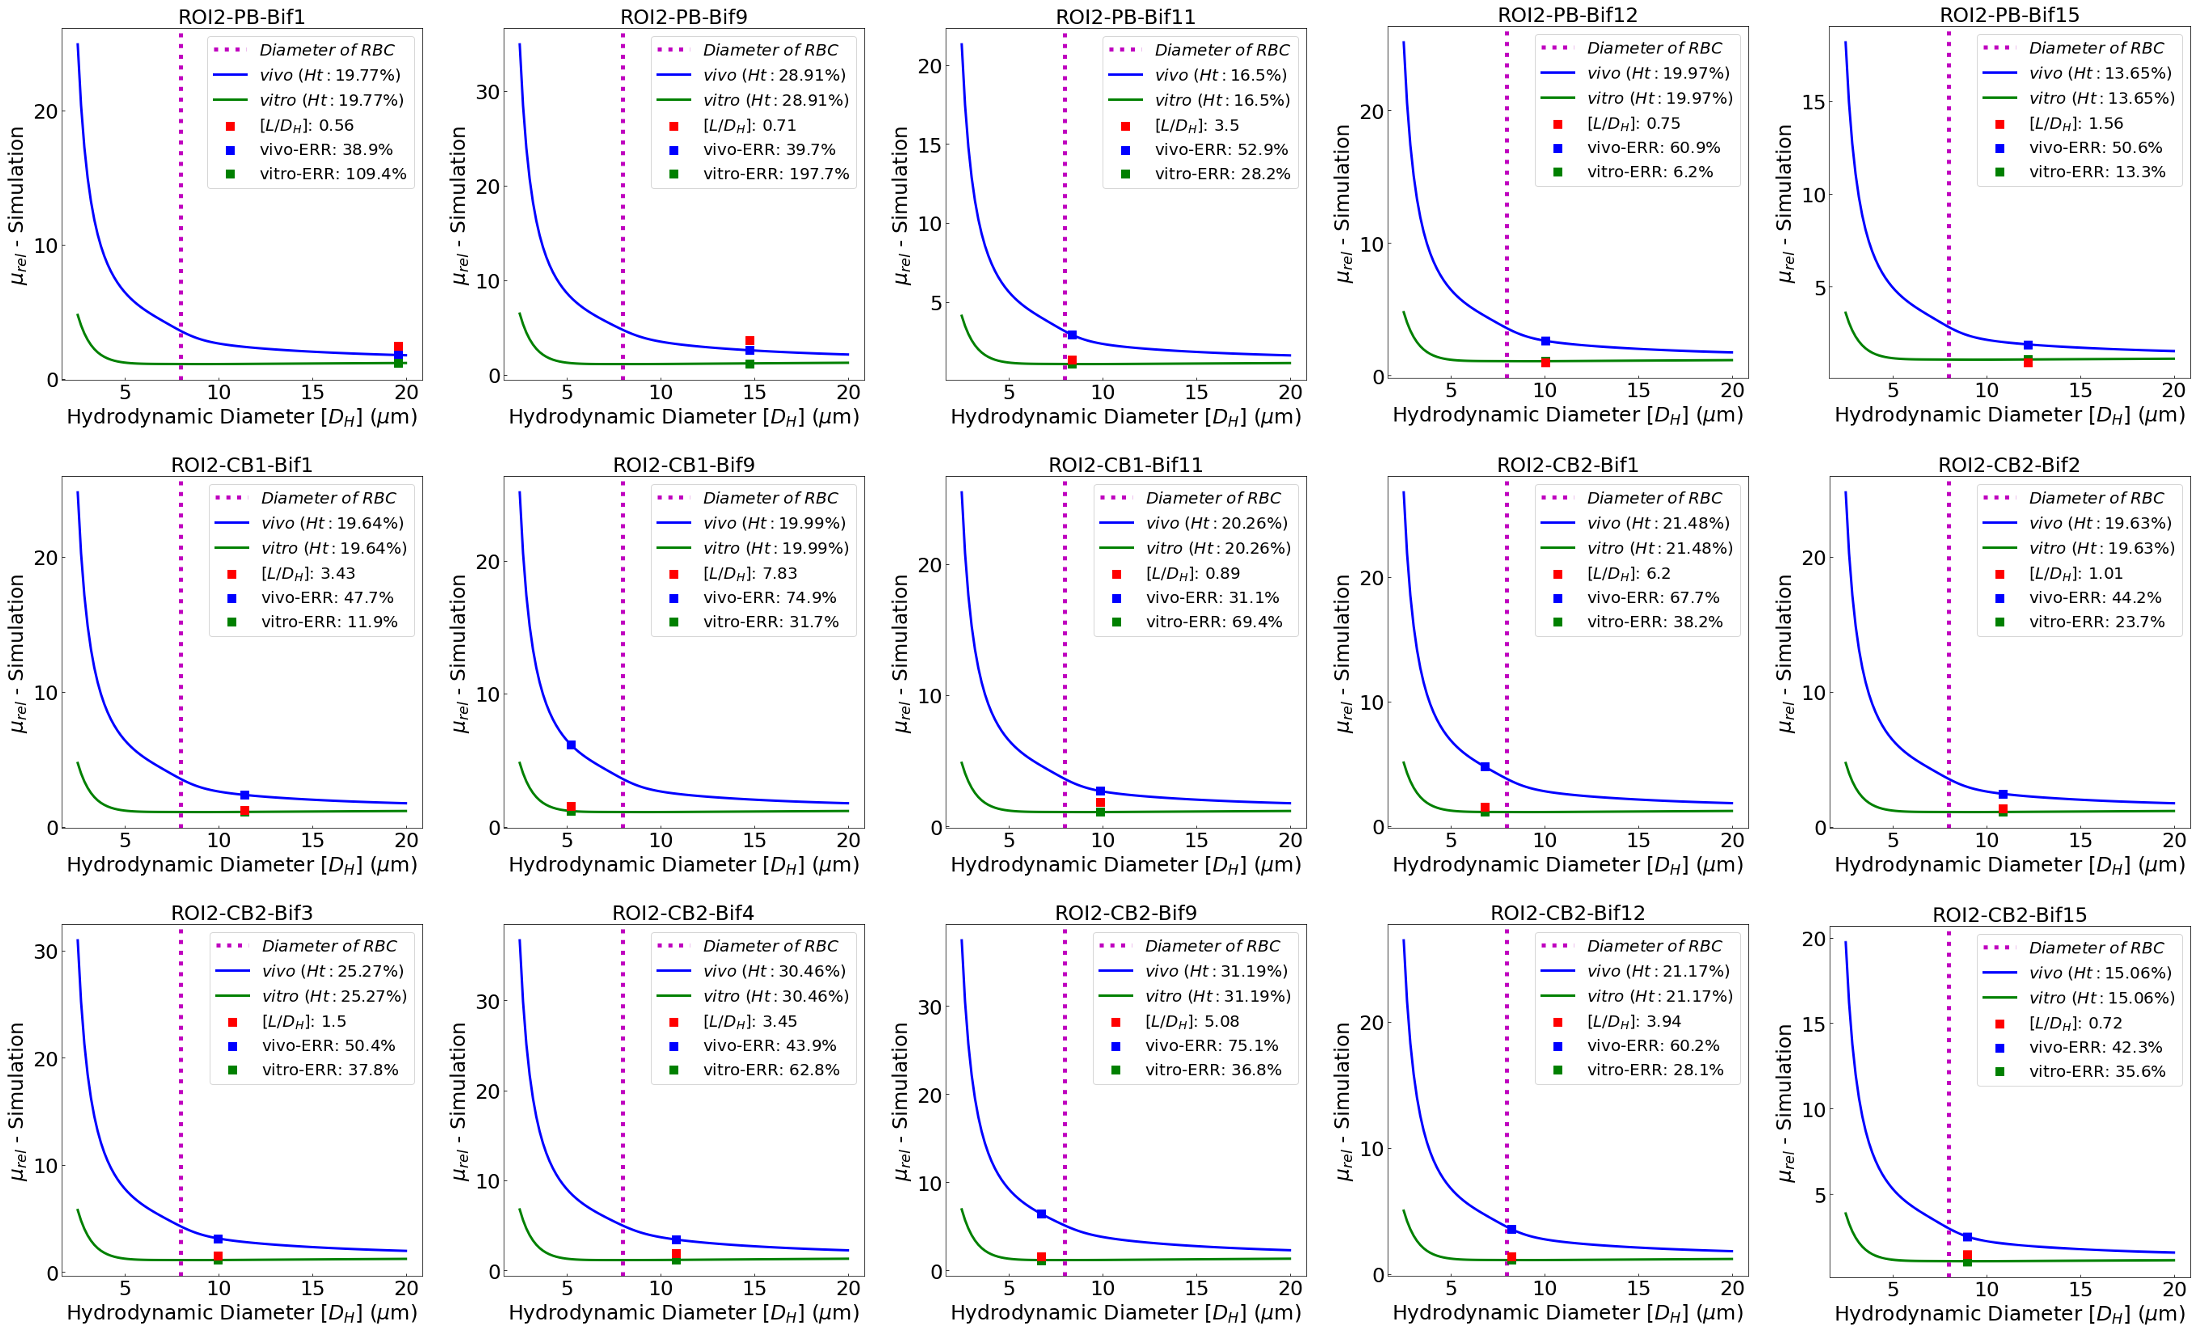
\includegraphics[width=0.95\textwidth]{images/DeviationsViscosity-ROI2.png}
\caption{\textit{Evaluation of non-zero haematocrit simulation data (red) against the empirical predictions (blue and green) from both in vivo and in vitro Pries Viscosity Models (solid lines) expressed as relative apparent viscosity ($\mu_{rel}$) against diameter (D$_{H}$) for each individual branch in ROI-2.(see Figure \ref{ROIs}b) The purple dotted line indicates the average diameter of a human RBC.} \label{DeviationsViscosity-ROI2}}
\end{figure}

\begin{figure}[H]
\centering
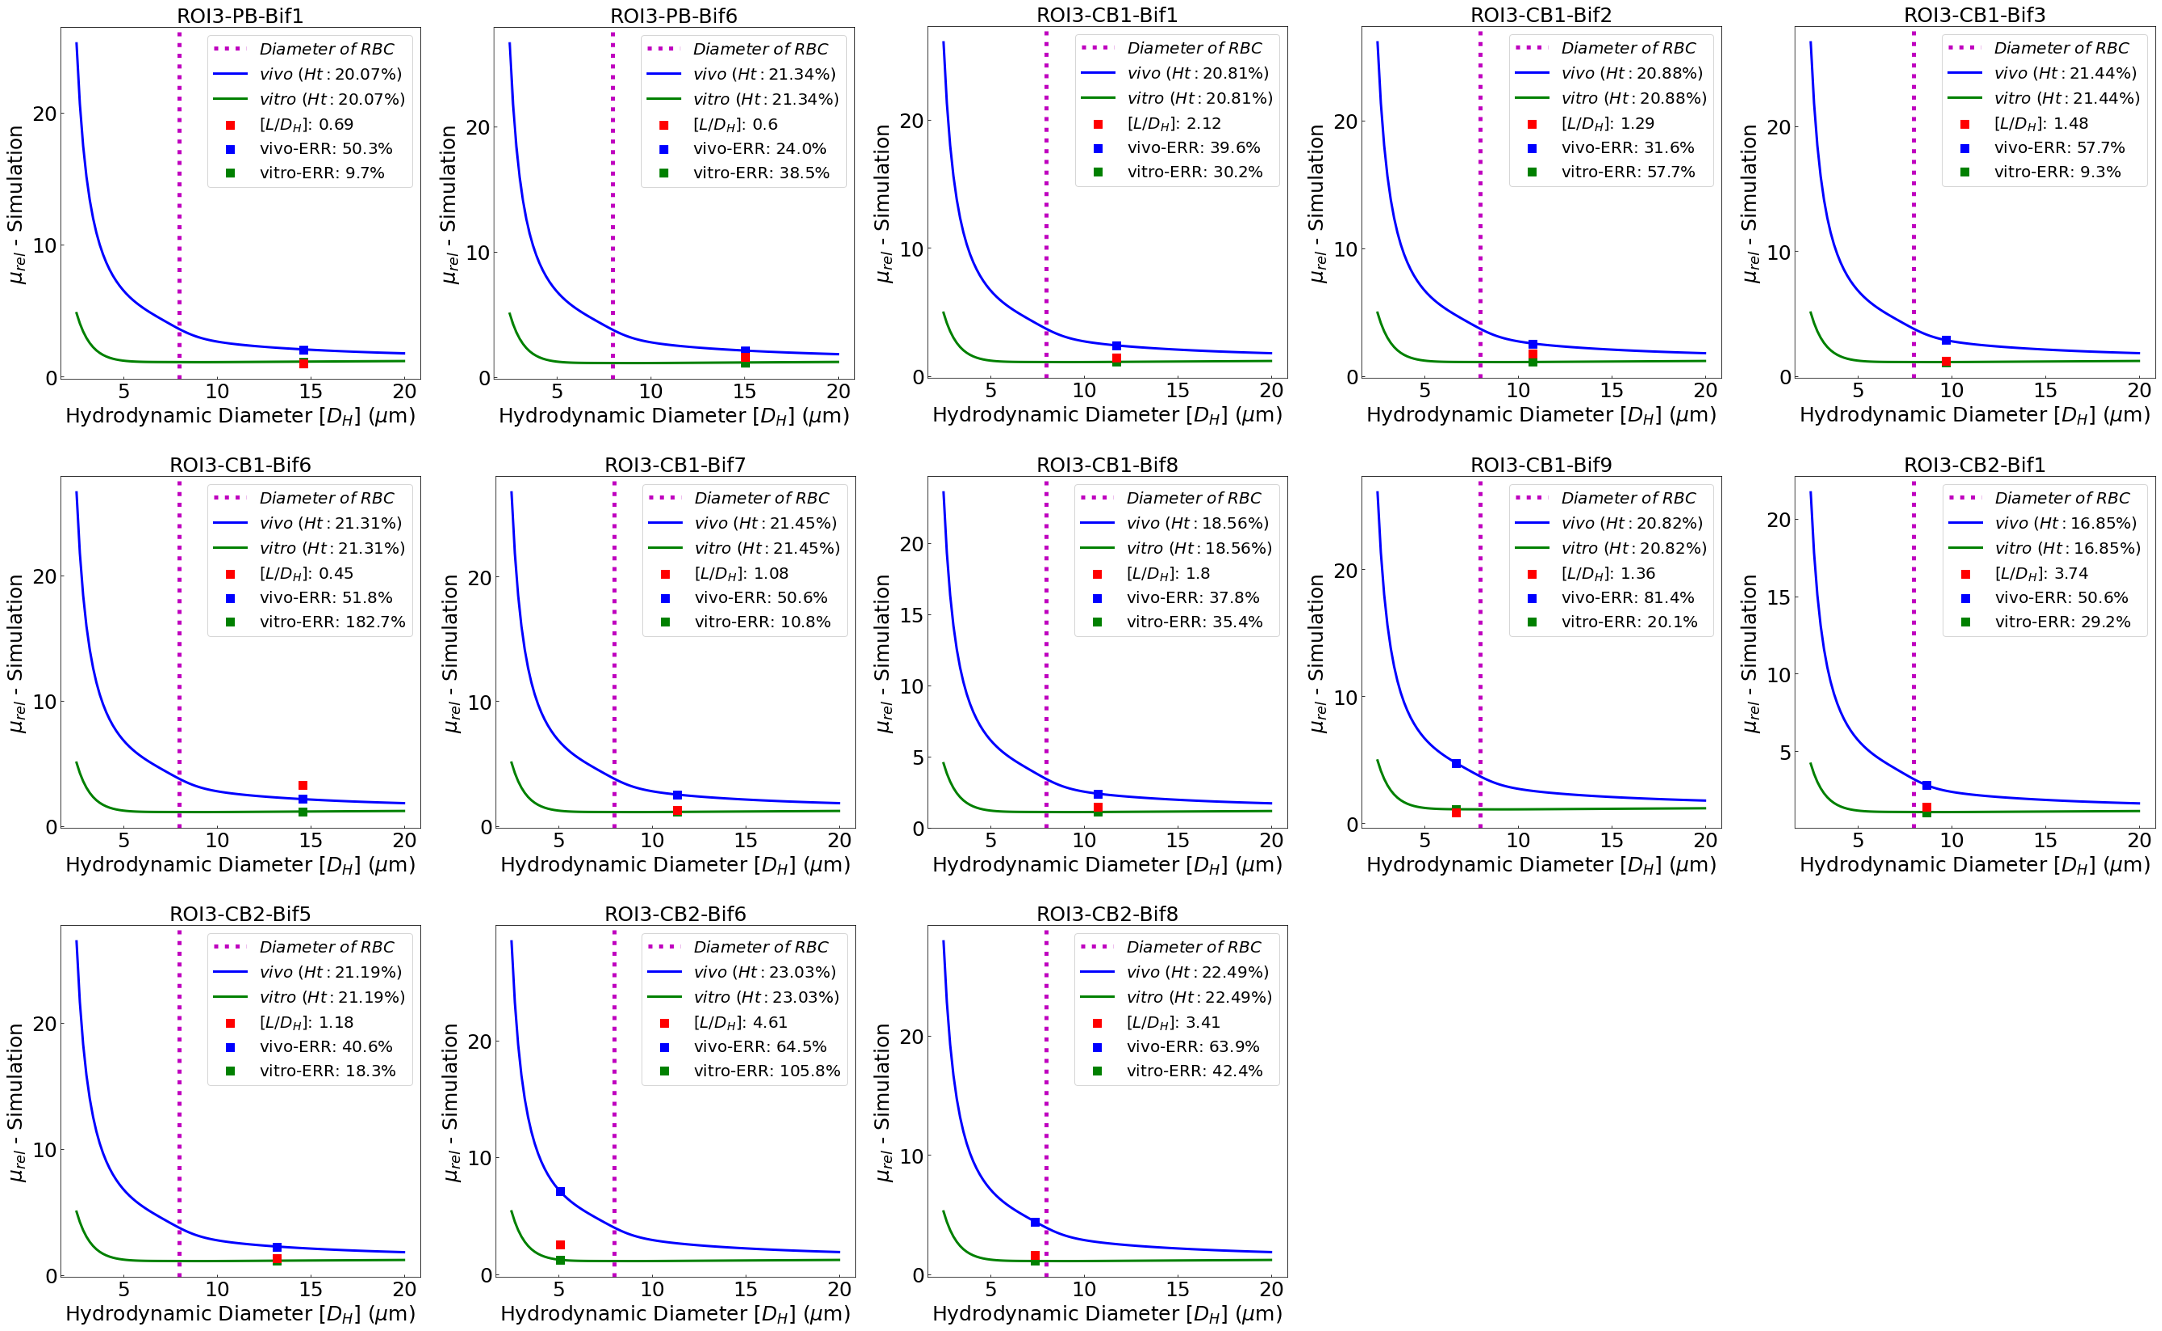
\includegraphics[width=0.95\textwidth]{images/DeviationsViscosity-ROI3.png}
\caption{\textit{Evaluation of non-zero haematocrit simulation data (red) against the empirical predictions (blue and green) from both in vivo and in vitro Pries Viscosity Models (solid lines) expressed as relative apparent viscosity ($\mu_{rel}$) against diameter (D$_{H}$) for each individual branch in ROI-3.(see Figure \ref{ROIs}c) The purple dotted line indicates the average diameter of a human RBC.} \label{DeviationsViscosity-ROI3}}
\end{figure}


\useportrait